\documentclass[oupdraft]{sysbio}
% \usepackage[colorlinks=true, urlcolor=citecolor, linkcolor=citecolor, citecolor=citecolor]{hyperref}

\usepackage{indentfirst}
\usepackage{url}
\usepackage{lipsum}
\usepackage{graphicx}
\usepackage{natbib}

% Add history information for the article if required
%\history{Received Month X, 20XX;
%revised Month X, 20XX}

\begin{document}

% Title of paper
\title{Lagrange-ng: The next generation of Lagrange}
% Each important word in the title should begin with a capital letter

% List of authors, with corresponding author marked by asterisk
\author{Ben Bettisworth$^{1,\ast}$, Stephen Smith$^{2}$, and
  Alexandros Stamatakis$^{1}$\\[4pt]
  % Author addresses
  \textit{$^{1}$~Computational Molecular Evolution Group, Heidelberg Institute for Theoretical Studies, Heidelberg,
    Germany}
  \\
  \textit{$^{2}$~Department, Institution, City, Post Code, Country}
  \\[2pt]
  % E-mail address for correspondence
  \textit{*Please direct all correspondence to \url{ben.bettisworth@h-its.org}}}
% Identify the name, address, telephone/fax numbers, and e-mail address for the author who will receive proofs and be designated the "corresponding author" in text.

% Running headers
\markboth%
{Ben Bettisworth}
{Lagrange-NG}

\maketitle

\begin{abstract}
  {}
  {Biogeography, Phylogenetics}
\end{abstract}
\newline

The dispersal-extinction-cladogenesis (DEC) model~\citep{ree_likelihood_2005} is a widely used to analyze biogeographical
data. Computation of likelihoods using this model, however, is characterized by exponential growth in with the number of
regions under consideration. This is due to 2 factors: the regions are splayed into $2^r = s$ states; and computation of
the transition matrix is $\mathcal{O}(s^3)$. Putting these two facts together, the complexity of computing a single
evaluation of the DEC model is $\mathcal{O}((2^r)^3) = \mathcal{O}(2^{3r})$. In other words, computation of the
likelihood is exponential with respect to the number of regions at hand. Therefore, the major constraining parameter to
data analysis under the DEC model will be the number of regions.

However, just computing the likelihood of the DEC model is not the most expensive step for parameter inference. Instead,
computation of the transition matrix dominates the runtime, often accounting for 80\% or more of the runtime for a given
inference.  The transition matrix is computed via an operation known as the matrix exponential. If $Q$ is a rate matrix,
then the transition matrix $P = e^{tQ}$. Much effort has been spent finding the best way to compute this operation
\citep{moler_nineteen_2003}, but it still remains a challenging operation to compute efficiently and accurately.
Additionally, the DEC model is non-reversible (I.E. uses a non-symmetric rate matrix), which limits the possible methods
of computing the matrix exponential, usually to less precise methods.

So, the primary challenge to computing a likelihood using the DEC model is computing the matrix exponential quickly. In
this work, we present a software implementation of the DEC model which contains a custom tooled version of the matrix
exponential algorithm called scaled and squaring, which can be used to compute results using the DEC model. This
software is a nearly complete rewrite of the Lagrange software by \citet{ree_likelihood_2005}. Additionally, we have
implemented a task-based hybrid multi-threading approach, which will greatly accelerate analysis of datasets with many
taxa. Furthermore, we also improve the numerical stability of the original software, and fix a major bug which we
discovered during development (Personal communication with Smith). Finally, in order to ensure that we match the
original implementation, we implemented a novel method of comparing range distribution on trees, which is based on the
Wasserstein metric.

\bigskip
\section{Software Description}\label{sec:description}

Lagrange-ng is an almost complete rewrite of the original (unpublished) C++ version of Lagrange. As such, Lagrange-ng
retains all the functionality of Lagrange, but does it more efficiently, and also implements a parallel version of the
same model. Improvements to Lagrange fall into one of 3 broad categories. First and largest is the support for parallel
computing, via a hybrid task based scheme. The second category includes the use of more efficient numerical methods,
including a custom tuned version of the matrix exponential. Third and final, there are the general improvements and
optimizations, which individually don't account for much of the efficiency gain, but together amount to a substantial
improvement. A thorough explanation of the software can be found in the supplementary material.

Lagrange-ng can be downloaded from GitHub at \url{https://github.com/computations/lagrange-ng}. To build the software,
the only dependencies are a C++ compiler, and CMake. Optionally, Lagrange-ng can be built with the system versions of
OpenBLAS \citep{openblas} and NLOpt \citep{nelder_simplex_1965, johnson_stevengjnlopt_2021}. Tests and tooling for
Lagrange-ng are written in Python 3 \citep{python3}, with additional support from Numpy \citep{numpy}, SciPy
\citep{scipy}, and seaborn \citep{Waskom2021}.

\bigskip
\section{Performance}\label{sec:performance}

In order to determine the performance of Lagrange-ng relative to the original implementation, we generated a large
number datasets randomly with a varying number of regions and ran either Lagrange or Lagrange-ng and recorded the
runtime. Each dataset had 100 taxa, and either 5, 6, or 7 regions. We generated 100 datasets for each parameter set of
taxa, regions and program. Furthermore, ran an additional series of performance evaluations on Lagrange-ng only with 8
threads assigned to coarse grained parallelization. The results of this performance are shown in
Figure~\ref{fig:all-results}.

\begin{figure}
  \noindent
  \begin{center}
    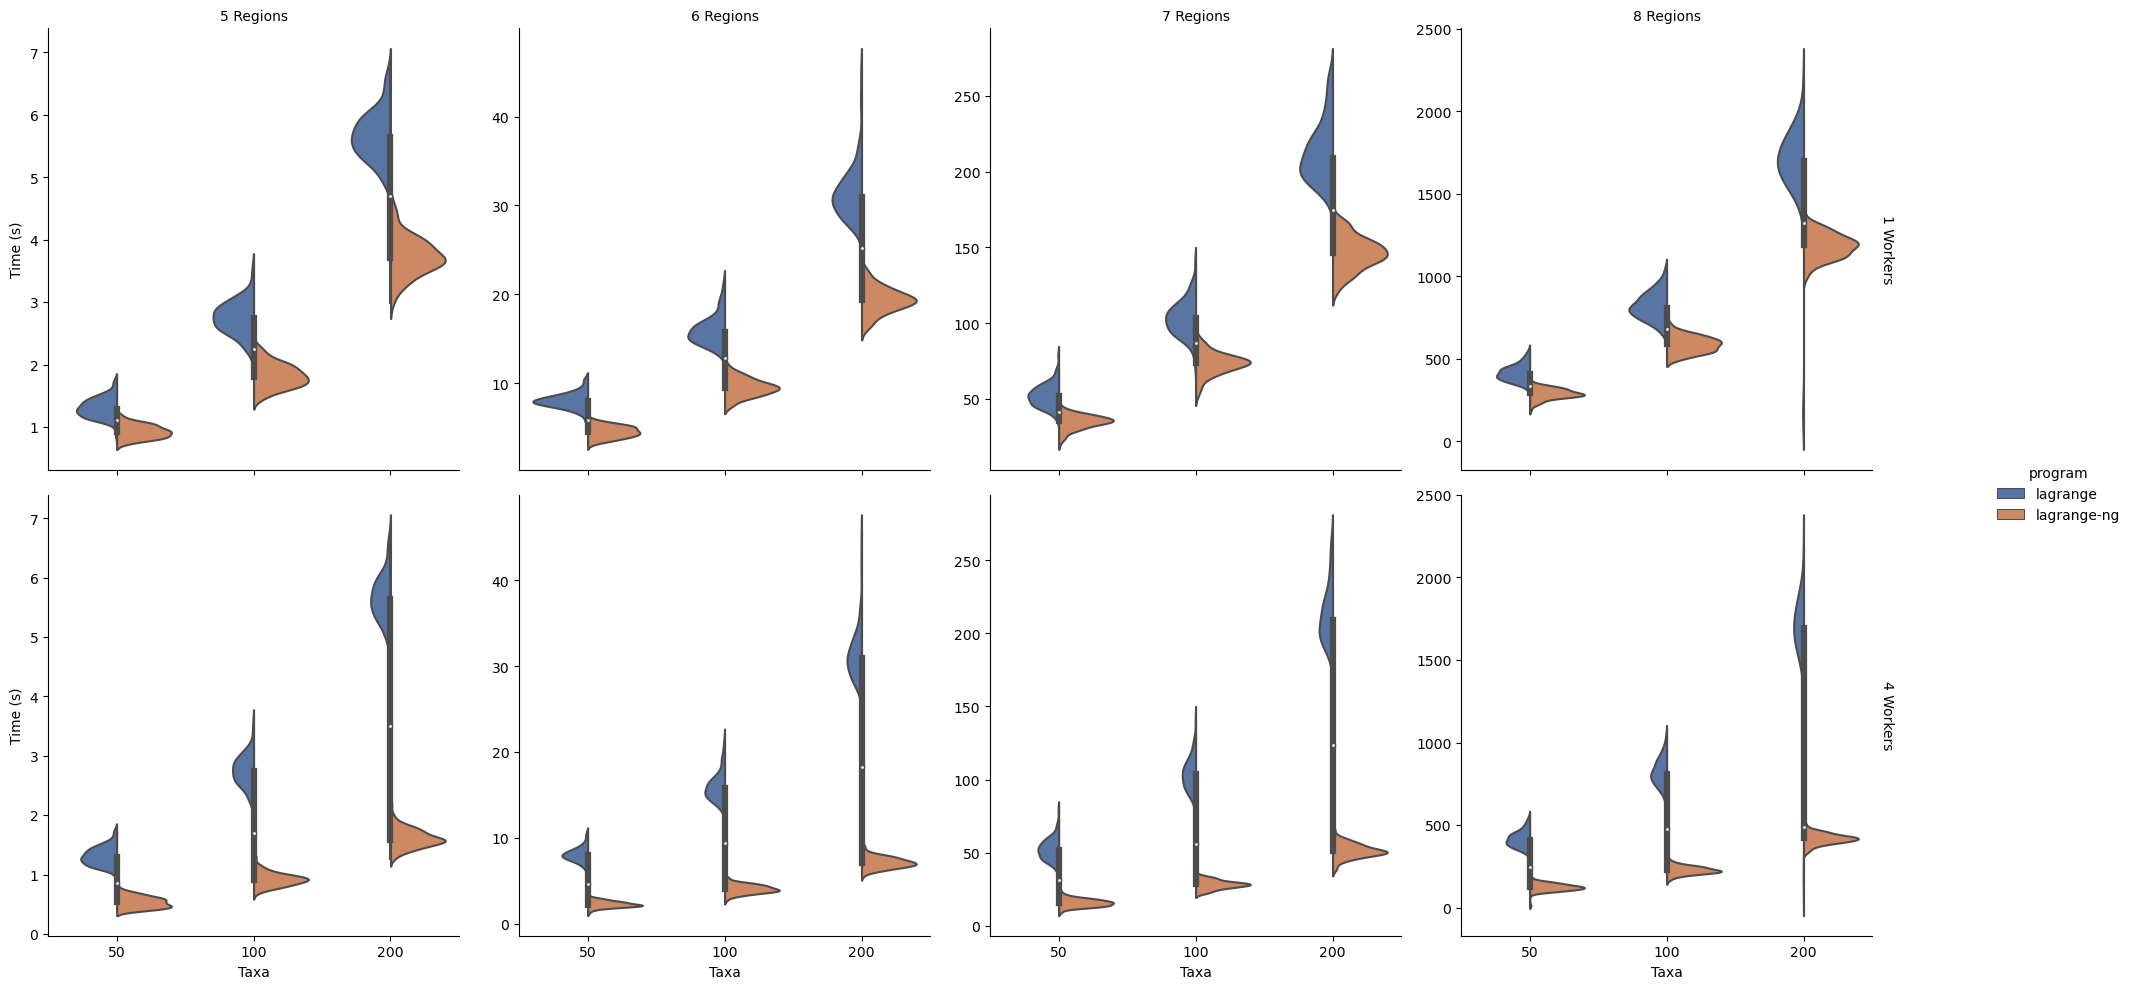
\includegraphics[width=\linewidth]{all_results_violin.png}
  \end{center}
  \caption{Comparision of runtimes between lagrange (left) and lagrange-ng (right) with lagrange-ng not using workers
    (top) and using 8 workers (bot). Results were obtained by generating 100 datasets randomly. Each program was given a
    different set of datasets, including Lagrange-ng with and without workers. Note that the original Lagrange was not
    run with workers, as it does not support them. Instead, the data has been replicated for comparison's sake. Time is
    in seconds. Figure was generated using seaborn \citep{Waskom2021}
    \label{fig:all-results}
  }
\end{figure}

\bigskip

\section{Validation}\label{sec:Validation}

Lagrange-ng replaces core numerical routines of Lagrange. Changes in numerical routines are often associated with
difficult and subtle bugs. We sought to ensure that Lagrange-ng and Lagrange produced the same results. To this end, we
developed both a pipeline to generate random datasets, run both Lagrange-ng and Lagrange, and compare the results of the
two programs. To compare results, we developed a distance to evaluate between distributions on trees based on the
Wasserstein metric \citep{vaserstein_markov_1969}. The details of how to calculate the metric are in the Supplementary
material. Nonetheless, we give a summary here.

To compute the distance between two ancestral range distributions for a given tree, embed the range into a hypercube
graph, and then use that graph to compute the Wasserstein metric between the distributions for each node. This metric is
then normalized to be between 0.0 and 1.0 by dividing by the maximum total distance, and then averaged over all nodes.
This method has the property that it accurately reflects the transitions between states in the DEC model.

We use this metric to ensure that Lagrange-ng obtains the same results for the same input as Lagrange (at least as much
as possible). We do this by randomly generating datasets (both trees and extant range distributions) for a given number
of taxa and ranges, and then running Lagrange to obtain the ground truth. From there, we run Lagrange-ng on the same
dataset, compute the results, and then ensure that the computed distance is below $1\times 10^{-4}$. However, some
datasets will yield different results even with a very tight tolerance, due to the optimization routines finding a
different optimum. So, for datasets which result in distributions who's distance is over tolerance fail, we run a linear
regression on the inferred values for the dispersion rate and the extinction rate against the distribution distance. If
the result is ``legitimately'' different, then there should be a strong correlation. If there is not, then it indicates
that there is a bug.

We ran this comparison for 100 iterations on datasets created with 10, 50 and 100 taxa, and a number of regions between
2 and 6. This yielded 15 datasets, and 1,500 total tests.

\section{Biological Examples}\label{sec:bio-examples}

While we conducted extensive tests on simulated data, it is still important that we ensure Lagrange-ng performs
correctly on real world examples. To this end, we have reproduced the results from a previous study on sloths from
\citet{varela_phylogeny_2019}. Additionally, we took the opportunity to reproduce the results using the tools specified
in the paper as this gave us an opportunity to compare with BioGeoBEARS \citep{biogeobears}, a similar tool.

In order to reproduce results, we downloaded the supplementary data from the Dryad repository associated with the
publication. In order to run the analysis for both BioGeoBEARS and Lagrange-ng, we had to modify the data slightly. This
involved correcting some names so that they matched, and removing the outgroup from the tree. These modifications appear
to be in line with what the original authors must have done, because the results from both BioGeoBEARS and Lagrange-ng
matches the results reported in the paper. Both BioGeoBEARS and Lagrange-ng were run with the same dataset, and the same
number of cores on the same computer.

\section{Results}\label{sec:Results}

The validation of Lagrange-ng, when compared to Lagrange, is very successful, despite heavy modifications of nearly all
critical code paths. Of the 1,500 tests, 12 ($0.8\%$) produced results with differences over tolerance when computed
using our novel distance method. The linear regression for the tests over threshold yielded a correlation coefficient of
$0.99997$, indicating that the failed runs are a product of differing optimizations, and not bugs in the tool.

The ratio between mean runtimes for Lagrange and Lagrange-ng with 1 worker for 5, 6, and 7 regions is 1.15, 1.05, and
0.96, respectively. The ratio between Lagrange and Lagrange-ng with 8 workers for 5, 6, and 7 regions is 3.56, 4.01, and
3.97, respectively.

However, Lagarange-ng fairs much better when compared with BioGeoBEARS. On the biological example, Lagrange-ng computed
the result in about $1$ minute, while BioGeoBEARS took about $24$ minutes to analyze the data. BioGeoBEARS and
Lagrange-ng inferred different optima for model parameters, with BioGeoBEARS achieving a slightly better likelihood
score. However, this hasn't affected the qualitative results when comparing between the two tools. This is to say,
BioGeoBEARS and Lagrange-ng both agree on the most likely distribution for every node.

\section{Discussion}\label{sec:Discussion}

We have shown that computation of biogeographical models can be greatly accelerated without a loss in quality of
results. A 4 fold increase in speed over the original implementation, and a 24 fold increase in speed over BioGeoBEARS
is very good. However, the parallel efficiency of 0.5 is disappointing. However, as detailed in the Supplementary
Material, the efficiency increases as the number of taxa increases. This means that as datasets get more taxa rich, and
run-times increase, Lagrange-ng will utilize it's computational resources more efficiently.

Future work on Lagrange-ng includes extending the range of models that can be computed to the DIVA and BAYAREA family of
models CITE THESE MODELS. Additionally, there is further work to be done optimizing the execution of the current models.
There are three areas in which the current performance can be improved upon, though we expect the benefits to be
marginal in most cases.

The first is to do a thorough exploration of the available BLAS implementations to determine which has the best
performance for this particular use case. While developing Lagrange-ng, we tried many different BLAS implementations,
but we did not do a complete investigation as to which had the best performance for the expected datasets. The second is
to further refine the matrix exponential routine. While we settled on a particular implementation with good performance,
there are other, more exotic methods which might yield better performance. Third is to further refine the work
allocation for the coarse grained parallelization. The current method of assigning tasks is quite na\"ive, and can be
improved upon by becoming aware of which nodes are "most blocking" of other tasks. It might be possible to devise an
algorithm that can minimize the "task starved" period of computation.

\bigskip

\section{Availability}\label{sec:availability}

The software, tools, and data used for this paper are available online at
\url{https://github.com/computations/lagrange-ng}.

\section{Supplementary Material}

\bigskip\bigskip

\bibliographystyle{unsrtnat}
\bibliography{references}

\end{document}
